% This file was created with tikzplotlib v0.10.1.
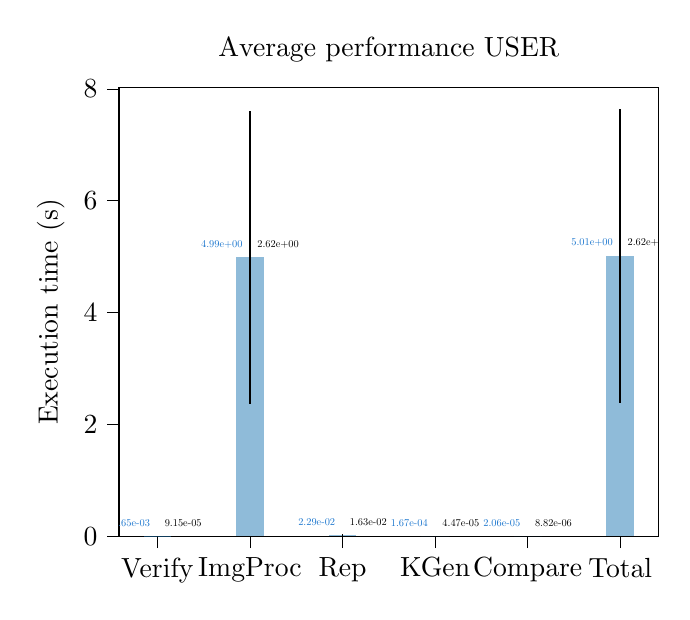
\begin{tikzpicture}

\definecolor{darkgray176}{RGB}{176,176,176}
\definecolor{royalblue24116205}{RGB}{24,116,205}
\definecolor{steelblue31119180}{RGB}{31,119,180}

\begin{axis}[
tick align=outside,
tick pos=left,
title={Average performance
USER},
x grid style={darkgray176},
xmin=-0.415, xmax=5.415,
xtick style={color=black},
xtick={0,1,2,3,4,5},
xticklabels={Verify,ImgProc,Rep,KGen,Compare,Total},
y grid style={darkgray176},
ylabel={Execution time (s)},
ymin=0, ymax=8.01761037123687,
ytick style={color=black}
]
\draw[draw=none,fill=steelblue31119180,fill opacity=0.5] (axis cs:-0.15,0) rectangle (axis cs:0.15,0.00164638857046758);
\draw[draw=none,fill=steelblue31119180,fill opacity=0.5] (axis cs:0.85,0) rectangle (axis cs:1.15,4.98634150743484);
\draw[draw=none,fill=steelblue31119180,fill opacity=0.5] (axis cs:1.85,0) rectangle (axis cs:2.15,0.0228689457972844);
\draw[draw=none,fill=steelblue31119180,fill opacity=0.5] (axis cs:2.85,0) rectangle (axis cs:3.15,0.000167359312375339);
\draw[draw=none,fill=steelblue31119180,fill opacity=0.5] (axis cs:3.85,0) rectangle (axis cs:4.15,2.06029415130615e-05);
\draw[draw=none,fill=steelblue31119180,fill opacity=0.5] (axis cs:4.85,0) rectangle (axis cs:5.15,5.01254164397717);
\path [draw=black, semithick]
(axis cs:0,0.00155485948767801)
--(axis cs:0,0.00173791765325716);

\path [draw=black, semithick]
(axis cs:1,2.36952971770451)
--(axis cs:1,7.60315329716517);

\path [draw=black, semithick]
(axis cs:2,0.00657277360014599)
--(axis cs:2,0.0391651179944228);

\path [draw=black, semithick]
(axis cs:3,0.000122619255267304)
--(axis cs:3,0.000212099369483375);

\path [draw=black, semithick]
(axis cs:4,1.17819100239749e-05)
--(axis cs:4,2.9423973002148e-05);

\path [draw=black, semithick]
(axis cs:5,2.38926388677636)
--(axis cs:5,7.63581940117797);

\draw (axis cs:0.04,0.00164638857046758) ++(0pt,2pt) node[
  scale=0.375,
  anchor=south west,
  text=black,
  rotate=0.0
]{9.15e-05};
\draw (axis cs:-0.04,0.00164638857046758) ++(0pt,2pt) node[
  scale=0.375,
  anchor=south east,
  text=royalblue24116205,
  rotate=0.0
]{1.65e-03};
\draw (axis cs:1.04,4.98634150743484) ++(0pt,2pt) node[
  scale=0.375,
  anchor=south west,
  text=black,
  rotate=0.0
]{2.62e+00};
\draw (axis cs:0.96,4.98634150743484) ++(0pt,2pt) node[
  scale=0.375,
  anchor=south east,
  text=royalblue24116205,
  rotate=0.0
]{4.99e+00};
\draw (axis cs:2.04,0.0228689457972844) ++(0pt,2pt) node[
  scale=0.375,
  anchor=south west,
  text=black,
  rotate=0.0
]{1.63e-02};
\draw (axis cs:1.96,0.0228689457972844) ++(0pt,2pt) node[
  scale=0.375,
  anchor=south east,
  text=royalblue24116205,
  rotate=0.0
]{2.29e-02};
\draw (axis cs:3.04,0.000167359312375339) ++(0pt,2pt) node[
  scale=0.375,
  anchor=south west,
  text=black,
  rotate=0.0
]{4.47e-05};
\draw (axis cs:2.96,0.000167359312375339) ++(0pt,2pt) node[
  scale=0.375,
  anchor=south east,
  text=royalblue24116205,
  rotate=0.0
]{1.67e-04};
\draw (axis cs:4.04,2.06029415130615e-05) ++(0pt,2pt) node[
  scale=0.375,
  anchor=south west,
  text=black,
  rotate=0.0
]{8.82e-06};
\draw (axis cs:3.96,2.06029415130615e-05) ++(0pt,2pt) node[
  scale=0.375,
  anchor=south east,
  text=royalblue24116205,
  rotate=0.0
]{2.06e-05};
\draw (axis cs:5.04,5.01254164397717) ++(0pt,2pt) node[
  scale=0.375,
  anchor=south west,
  text=black,
  rotate=0.0
]{2.62e+00};
\draw (axis cs:4.96,5.01254164397717) ++(0pt,2pt) node[
  scale=0.375,
  anchor=south east,
  text=royalblue24116205,
  rotate=0.0
]{5.01e+00};
\end{axis}

\end{tikzpicture}
